\documentclass[10pt]{beamer}
% \documentclass[handout,10pt]{beamer}
\usepackage{my_style}
%%%%%%%%%%%%%%%%%%%%%%%%%%%%%%%%%%%%%%%%%%%%%%%%%%%%%%%%%%%%%%%%%%%%%%%%
%%%%%%%%%%%%%%%%%%%%%%%%%%%%%%%%%%%%%%%%%%%%%%%%%%%%%%%%%%%%%%%%%%%%%%%%

\title[Math/CS 375]{Lecture 14 - B}
\subtitle{\S 9.1 Least-Squares}

\begin{document}
% -------------------------------------------------
\begin{frame}
  \titlepage
\end{frame}

%%%%%%%%%%%%%%%%%%%%%%%%%%%%%%%%%%%%%%%%%%%
\begin{frame}{Goals}
We will answer these questions:\\[3mm]
\begin{itemize}
    \item How is SVD used for semantic analysis?
    \item What is an overdetermined system and when does it arise in applications?
    \item What is the standard way to solve an overdetermined system?
    \item How can you use the SVD to solve overdetermined systems and why?
\end{itemize}
\end{frame}

%%%%%%%%%%%%%%%%%%%%%%%%%%%%%%%%%%%%%%%%%%%%%%%%%%%%
\sectionframe{Semantic Analysis}
%%%%%%%%%%%%%%%%%%%%%%%%%%%%%%%%%%%%%%%%%%%%%%%%%%%%

\begin{frame}{Too Much Text}

\begin{itemize}
\item Suppose we collect hundreds of thousands of customer reviews:
\end{itemize}

\vspace{2mm}

\begin{block}{Examples}
\begin{itemize}
\item "game is fun for kids"
\item "does not work on mac"
\item "installation failed on windows"
\item "kids love this game"
\end{itemize}
\end{block}

\vspace{3mm}

\pause

\question{
Can we automatically understand what people are talking about?
}
\end{frame}
%%%%%%%%%%%%%%%%%%%%%%%%%%%%%%%%

\begin{frame}{Idea}

\begin{itemize}
\item We want to find patterns in how words appear
\item Words that appear together may represent a "topic"
\end{itemize}

\vspace{4mm}

\keyidea{
We will turn text into numbers and let linear algebra find structure.
}

\end{frame}
%%%%%%%%%%%%%%%%%%%%%%%%%%%%%%%%
\begin{frame}{Document-Word Matrix}


\begin{center}
\begin{tabular}{c|cccc}
 & game & kids & mac & install \\
\hline
Doc 1 & 1 & 1 & 0 & 0 \\
Doc 2 & 0 & 0 & 1 & 0 \\
Doc 3 & 0 & 0 & 0 & 1 \\
Doc 4 & 1 & 1 & 0 & 0 \\
\end{tabular}
\end{center}

\vspace{3mm}

\begin{itemize}
\item Load every document and create a list of unique words
\item After preprocessing (e.g. stemming installation to install), record word presence with 1s and 0s
\item Each row = a document
\item Each column = a word
\end{itemize}

\end{frame}
%%%%%%%%%%%%%%%%%%%%%%%%%%%%%%%%
\begin{frame}{Apply SVD}

\[
A = U \Sigma V^T
\]

\vspace{3mm}

\begin{itemize}
\item Columns of $V$ give orthonormal word patterns
\item The singular values in $\Sigma$ rank the strength of these patterns
\item Rows of $U\Sigma=AV$ give each document's coefficients in this basis
\end{itemize}

\end{frame}
%%%%%%%%%%%%%%%%%%%%%%%%%%%%%%%%
\begin{frame}{Example}

\begin{figure}
    \centering
    
\includegraphics[width=0.6\linewidth]{figs/word_cloud.png}
\end{figure}

\begin{itemize}
    \item 2018 Amazon customer reviews in the Video Games category
    \item 497,577 total reviews
    \item Source: \texttt{https://nijianmo.github.io/amazon/index.html}
\end{itemize}
\end{frame}
%%%%%%%%%%%%%%%%%%%%%%%%%%%%%%%%
\begin{frame}{Result}
\begin{itemize}
    \item Each right singular vector contains signed weights for the vocabulary words
% For a reproducible ranking, sort by absolute weight and inspect both signs.
% These previously reported lists are retained; their ranking convention is unverified.

    \item Reported words from $v_1$:
    $$
    \text{
        "game"    "like"    "games"    "just"    "get"    "play"    "time"  
    }
    $$
    \item Reported words from $v_2$
    $$
    \text{"game"    "like"    "games"    "just"    "get"    "really"    "controller"}
    $$
    \item Reported words from $v_3$
    $$
    \text{"games"    "wii"    "just"    "play"    "get"    "like"    "mario"}
    $$
\end{itemize}
\begin{block}{Inference}
    Frequent generic words obscure the patterns. Word selection and preprocessing matter.
\end{block}
\end{frame}
%%%%%%%%%%%%%%%%%%%%%%%%%%%%%%%%
\begin{frame}[fragile]{New Result}

\begin{itemize}
\item Removed selected common words 
$$
\text{game, games, play, like, get, really, time}
$$

\item New result 
\begin{lstlisting}
Topic 1: good even first well story fun 

Topic 2: wii controller story link xbox characters 

Topic 3: link mario good class characters normal 

Topic 4: mario wii fun link super new 

Topic 5: great good fun story graphics even 
\end{lstlisting}
\end{itemize}

\begin{block}{Inference}
These patterns suggest themes, not established sentiment or popularity. For interpretation, rank words by absolute weight and examine positive and negative weights separately.
\end{block}

\end{frame}

%%%%%%%%%%%%%%%%%%%%%%%%%%%%%%%%

\begin{frame}{Big Idea}
\begin{itemize}
\item We never told the computer what a "topic" is
\item It identified word co-occurrence patterns that we can interpret
\end{itemize}

\vspace{4mm}

\keyidea{
SVD orders patterns by strength; interpreting them as topics requires judgment.
}
\end{frame}

%%%%%%%%%%%%%%%%%%%%%%%%%%%%%%%%%%%%%%%%%%%%%%%%%%%%
\sectionframe{Linear Regression}
%%%%%%%%%%%%%%%%%%%%%%%%%%%%%%%%%%%%%%%%%%%%%%%%%%%%


\begin{frame}{Regression vs Interpolation}
\cols{
    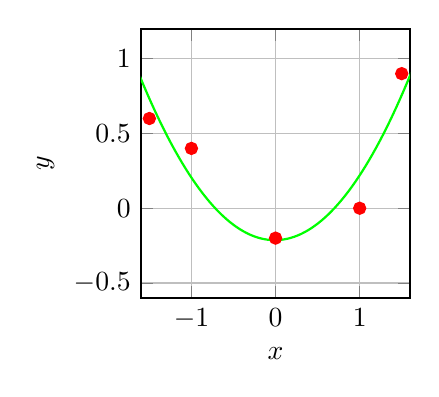
\begin{tikzpicture}
    \begin{axis}[
        width=5cm, height=5cm,
        xmin=-1.6, xmax=1.6, ymin=-0.6, ymax=1.2,
        xlabel={$x$}, ylabel={$y$},
        grid=major, 
        thick,
        domain=-2:2,
        samples=100,
        % legend pos=outer south
    ]
    % Regression curve (for example, a quadratic fit)
    \addplot[color=green, thick] {0.4258503401*x^2 + 0.0076923077*x - 0.2136054422};

    % Data points (scatter around the regression curve)
    \addplot[color=red, only marks, mark=*] 
        coordinates {(-1.5,0.6) (-1,0.4) (0, -0.2) (1, 0) (1.5, 0.9)};
    
    % Optional legend
    % \legend{Regression $g(x)$, Data Points};
    \end{axis}
    \end{tikzpicture}
}{
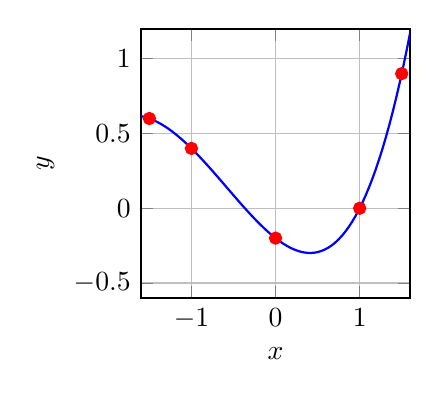
\begin{tikzpicture}
    \begin{axis}[
        width=5cm, height=5cm,
        xmin=-1.6, xmax=1.6, ymin=-0.6, ymax=1.2,
        xlabel={$x$}, ylabel={$y$},
        grid=major, 
        thick,
        domain=-2:2,
        samples=100,
        % legend pos=outer south
    ]
    % Degree-four interpolant through the same five data points
    \addplot[color=blue, thick] {0.01777777778*x^4 + 0.24*x^3 + 0.38222222222*x^2 - 0.44*x - 0.2};

    % Interpolation points
    \addplot[color=red, only marks, mark=*] 
        coordinates {(-1.5,0.6) (-1,0.4) (0,-0.2) (1,0) (1.5,0.9)};
    
    % Optional legend
    % \legend{Interpolation $g(x)$, Data Points};
    \end{axis}
\end{tikzpicture}\\
}

\begin{itemize}
    \item Both  extract continuous functions $f(x)$ from discrete data
    \item \textbf{Regression}: find a function that ``best" fits the data
    \item \textbf{Interpolation}: find a function that passes through all data points
\end{itemize}
\end{frame}



%%%%%%%%%%%%%%%%%%%%%%%%%%%%%%%%%%%%%%%%%%%%%%%%%%%%%%%%%%%%%%%%%%%%%%
\begin{frame}{Noise in Real data}
\begin{itemize}
    \item Real data $\{(x_1,y_1), ..., (x_n, y_n)\}$ contains noise (random error)
    \item Regression is more suitable than interpolation for noisy data
\end{itemize}

\begin{center}
  \pgfimage [width = 6cm] {figs/polling}
\end{center}
\end{frame}
%%%%%%%%%%%%%%%%%%%%%%%%%%%%%%%%%%%%%%%%%%%%%%%%%%%%%%%%%%%%%%%%%%%%%
% \begin{frame}{Noise in Simulated data}

% \cols{
% \begin{itemize}
%     \item We may produce data $\{(x_1,y_1), ..., (x_n, y_n)\}$ by sampling from some function $y = f(x)$\\[3mm]
%     \item We may introduce \emph{artificial} random error into our sampled data\\[3mm]
%     \item Use \texttt{randn} for Gaussian noise or \texttt{rand} for uniform noise
% \end{itemize}

% }{
% \begin{center}
%   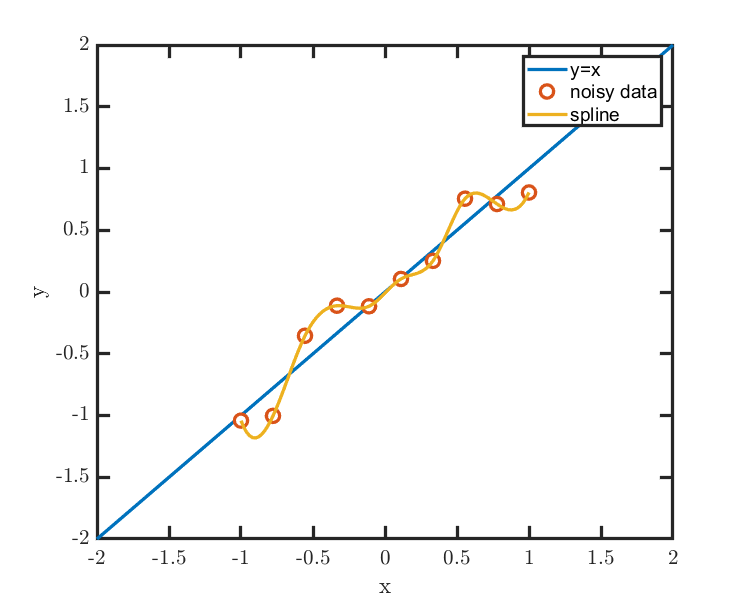
\includegraphics[scale=0.3] {figs/linear_interp}
% \end{center}
% }

% \question{
%     Can we recover the true solution $y=f(x)$ based using only the noisy data?
% }
% \end{frame}
%%%%%%%%%%%%%%%%%%%%%%%%%%%%%%%%%%%%%%%%%%%%%%%%%%%%%%%%%%%%%%%%%%%%%

\begin{frame}{Linear Regression}

\question{Here is a set of 20 noisy data points. How do you fit a line on the data?}
\begin{figure}
    \centering
    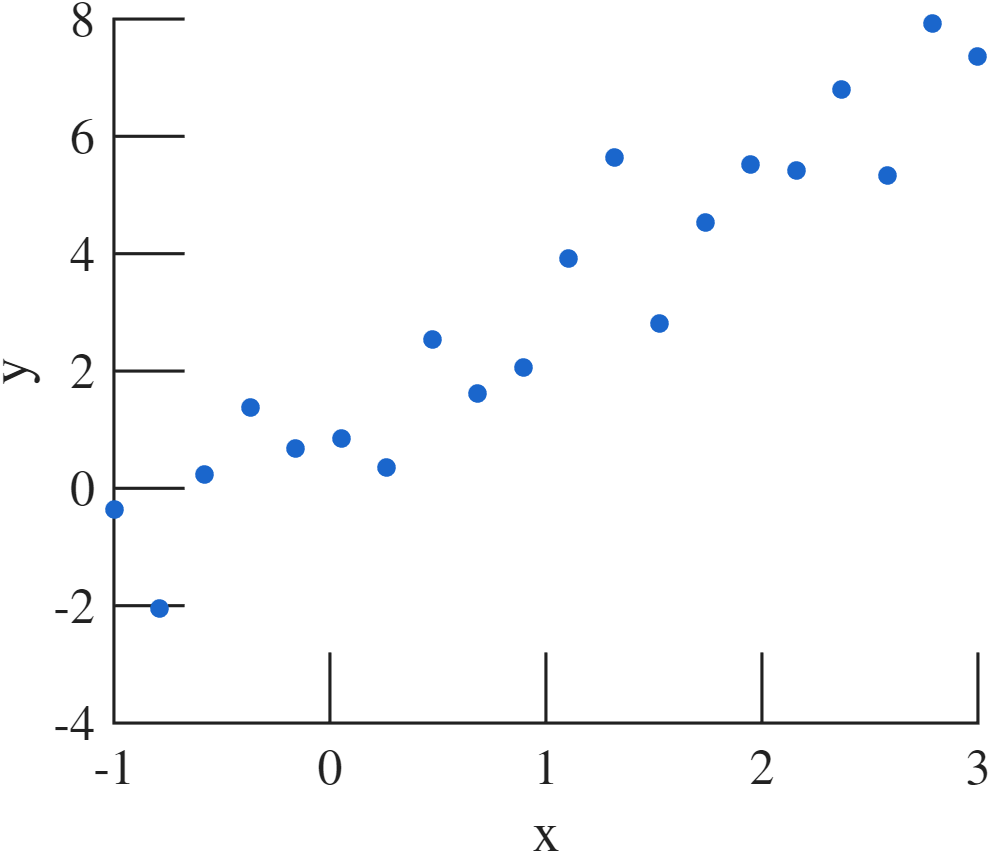
\includegraphics[width=0.5\linewidth]{figs/scatter.png}
\end{figure}


\end{frame}



%%%%%%%%%%%%%%%%%%%%%%%%%%%%%%%%%%%%%%%%%%%%%%%%%%%%%%%%%%%%%%%%%%%%%
\begin{frame}{Interpolation?}

\begin{block}{Interpolation Problem}
\begin{itemize}
\item Given: $n$ data points $\{(x_1,y_1),...,(x_n,y_n)\}$
\item Goal: Find a line $ y = \alpha x + \beta$ that fits through all $n$ points    
\end{itemize}
\end{block}
\vspace{3mm}

In matrix form
$$ \underbrace{\begin{bmatrix}x_1 & 1 \\ \vdots & \vdots \\x_n & 1 \end{bmatrix}}_A 
\underbrace{\begin{bmatrix}\alpha \\ \beta \end{bmatrix}}_{x} 
= 
\underbrace{\begin{bmatrix} y_1 \\ \vdots \\ y_n \end{bmatrix}}_{\mathbf{y}}$$
For $n>2$, the system is overdetermined; an exact solution requires all points to lie on a line $y=\alpha x+\beta$. 

\keyidea{
A line generally cannot pass through all twenty noisy data points.
}
\end{frame}

%%%%%%%%%%%%%%%%%%%%%%%%%%%%%%%%%%%%%%%%%%%%%%%%%%%%%%%%%%%%%%%%%
\begin{frame}{Overdetermined Problem}

The issue: generally $\mathbf{y}\notin\operatorname{Range}(A)$, so no line fits all the data exactly.


    \keyidea{
    \begin{itemize}
        \item \textbf{Give up} on trying to pass a line through all points 
        \item Find the \textbf{line of best fit} instead
    \end{itemize}
    }
    \bigskip
Let's rework the problem
    \begin{itemize}
    
    \item We still want a line $\hat{y}=\alpha x+\beta$
    \item We want our line to be optimal in some way
    \end{itemize}

    \question{What makes a line ``best fit''?}
\end{frame}

%%%%%%%%%%%%%%%%%%%%%%%%%%%%%%%%%%%%%%%%%%%%%%%%%%%%%%%%%%%%%%%%%
\begin{frame}{What is the best line?}

\begin{figure}
    \centering
    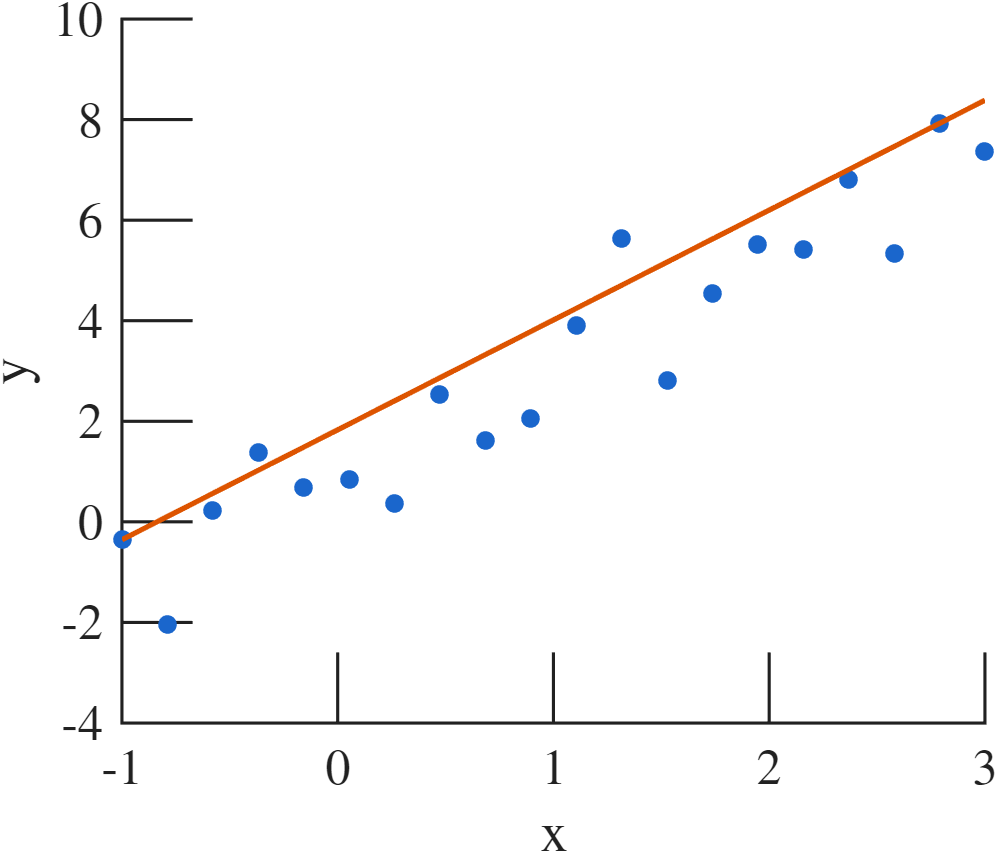
\includegraphics[width=0.5\linewidth]{figs/scatter2.png}
\end{figure}

\question{
\begin{itemize}
    \item Do you think this is the best line? 
    \item How can you tell?
    \item How can we quantify the goodness of the fit?
\end{itemize}
}
\end{frame}
%%%%%%%%%%%%%%%%%%%%%%%%%%%%%%%%%%%%%%%%%%%%%%%%%%%%%%%%%%%%%%%%%
\begin{frame}{Quantify the Error}

\begin{figure}
    \centering
    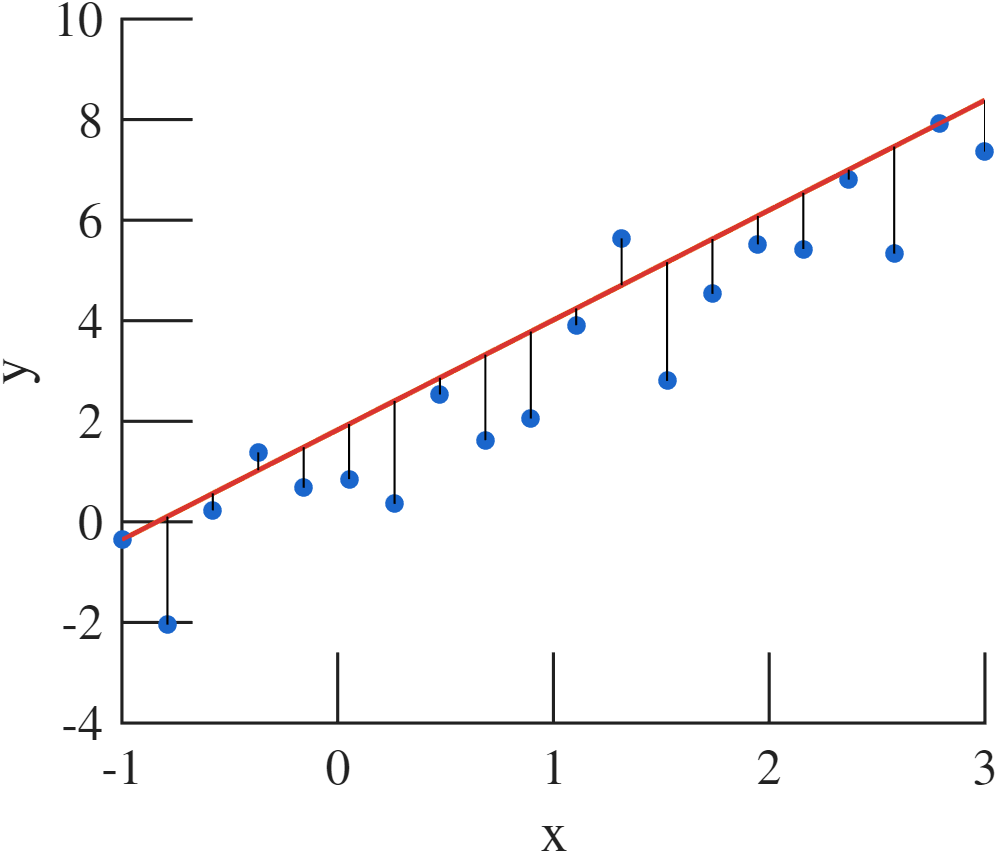
\includegraphics[width=0.5\linewidth]{figs/scatter3.png}
\end{figure}

\begin{itemize}
    \item For any line, we can add up the vertical error at each point
    \item We can define error to be 
    $$
        E =  \sum_i| \text{$i^{th}$ vertical bar|}^2
    $$
\end{itemize}
\end{frame}
%%%%%%%%%%%%%%%%%%%%%%%%%%%%%%%%%%%%%%%%%%%%%%%%%%%%%%%%%%%%%%%%%
\begin{frame}{The Residual}

\begin{itemize}

    \item The signed vertical difference is the \textbf{residual}
    $$
        r_i = y_i - (\alpha x_i+\beta)
    $$
    \item $r_i$ can be positive or negative. That's why we square them.
    \item The error is 
    $$
        E = \sum_i  (r_i)^2
    $$
    \item Since the matrix form is
    $$ \begin{bmatrix}x_1 & 1 \\ \vdots & \vdots \\x_n & 1 \end{bmatrix}
\begin{bmatrix}\alpha \\ \beta \end{bmatrix}
= 
\begin{bmatrix} y_1 \\ \vdots \\ y_n \end{bmatrix}$$
with $\mathbf{y}=(y_1,\ldots,y_n)^T$, the residual in \textbf{vector form} is
$$
\boxed{
    r = \mathbf{y} - Ax
}
$$
\end{itemize}
\end{frame}
%%%%%%%%%%%%%%%%%%%%%%%%%%%%%%%%%%%%%%%%%%%%%%%%%%%%%%%%%%%%%%%%%

%%%%%%%%%%%%%%%%%%%%%%%%%%%%%%%%%%%%%%%%%%%%%%%%%%%%%%%%%%%%%%%%%
\begin{frame}{Least Squares}
\begin{itemize}
\item In the general notation $Ax=b$, $b$ denotes the data vector.
\item Let $x$ represent a particular "fit" 
$$
x = \begin{bmatrix}
    \alpha\\\beta
\end{bmatrix}
$$
for the line $y=\alpha x+\beta$

\define{Residual and Squared Error}{
The {\bf{residual}} vector is  $$r = b-Ax.$$ 
The quantity $\|r\|_2^2$ is the \textbf{sum of squared residuals}.
}

\method{Least Squares}{Overdetermined system $Ax=b$}{Best approximate solution $x$}{Choose $x$ to minimize $\|b-Ax\|_2^2$.}

\end{itemize}
\end{frame}

%%%%%%%%%%%%%%%%%%%%%%%%%%%%%%%%%%%%%%%%%%%%%%%%%%%%%%%%%%%%%%%%%%.
\begin{frame}{Optimize}

\begin{figure}
    \centering
    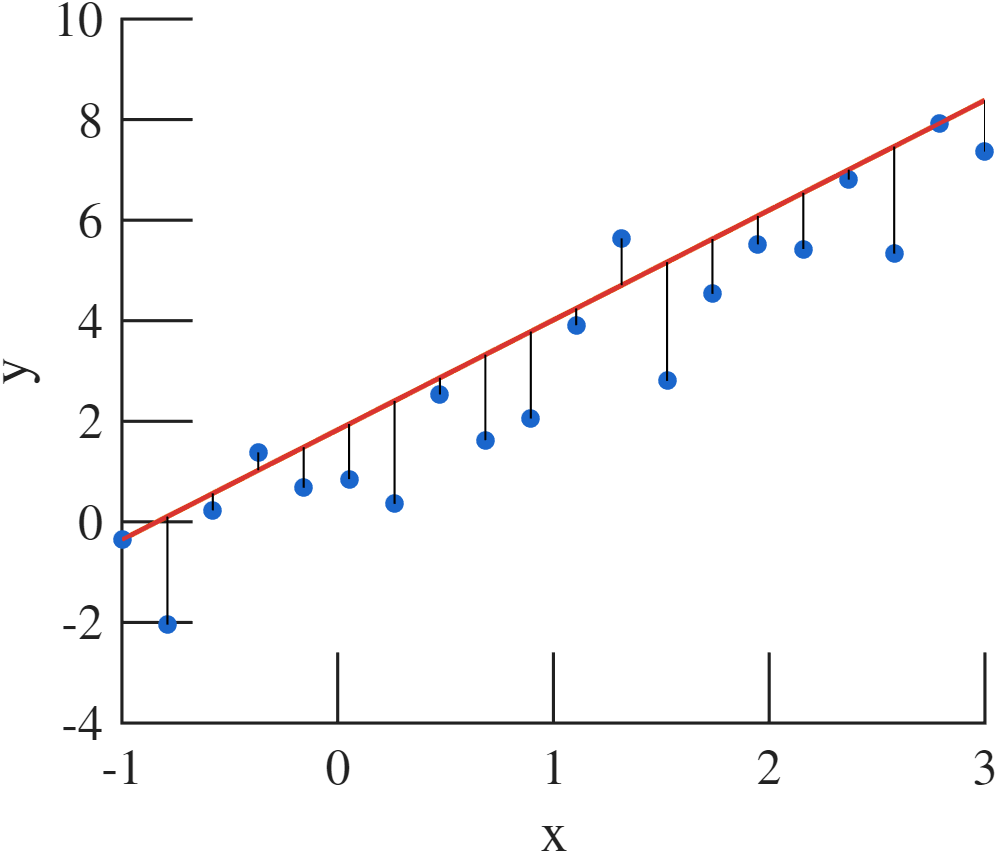
\includegraphics[width=0.5\linewidth]{figs/scatter3.png}
\end{figure}

\begin{itemize}
    \item For any fit $y=\alpha x+\beta$, we can compute the least squares error
    $$
        E =  \sum_i| \text{$i^{th}$ vertical bar|}^2 = \sum_i (r_i)^2 = r^Tr = \|r\|^2
    $$
    \item \textbf{Goal}: find the values $\alpha$ and $\beta$ that minimize the error

\end{itemize}
\end{frame}

%%%%%%%%%%%%%%%%%%%%%%%%%%%%%%%%%%%%%%%%%%%%%%%%%%%%%%%%%%%%%%%%%
\begin{frame}{Visual}

\cols{
\begin{figure}
    \centering
    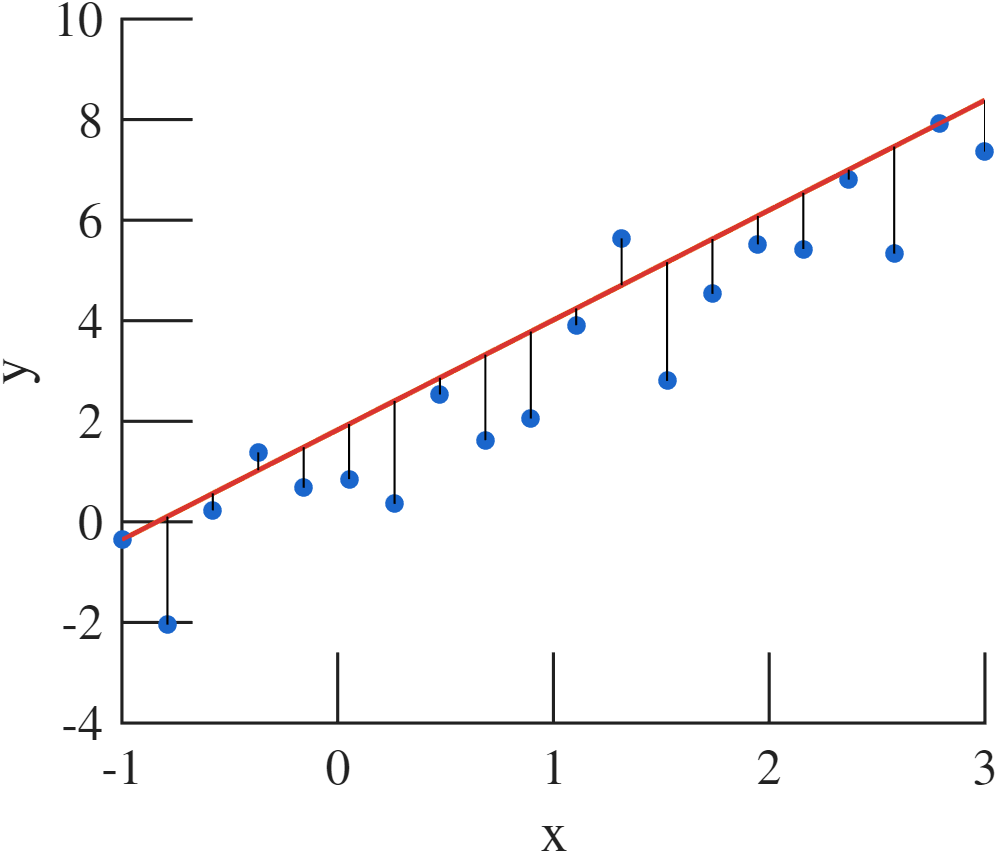
\includegraphics[width=\linewidth]{figs/scatter3.png}
    Sum of squared residuals $\|r\|_2^2=31.8624
$
\end{figure}
}{
\begin{figure}
    \centering
    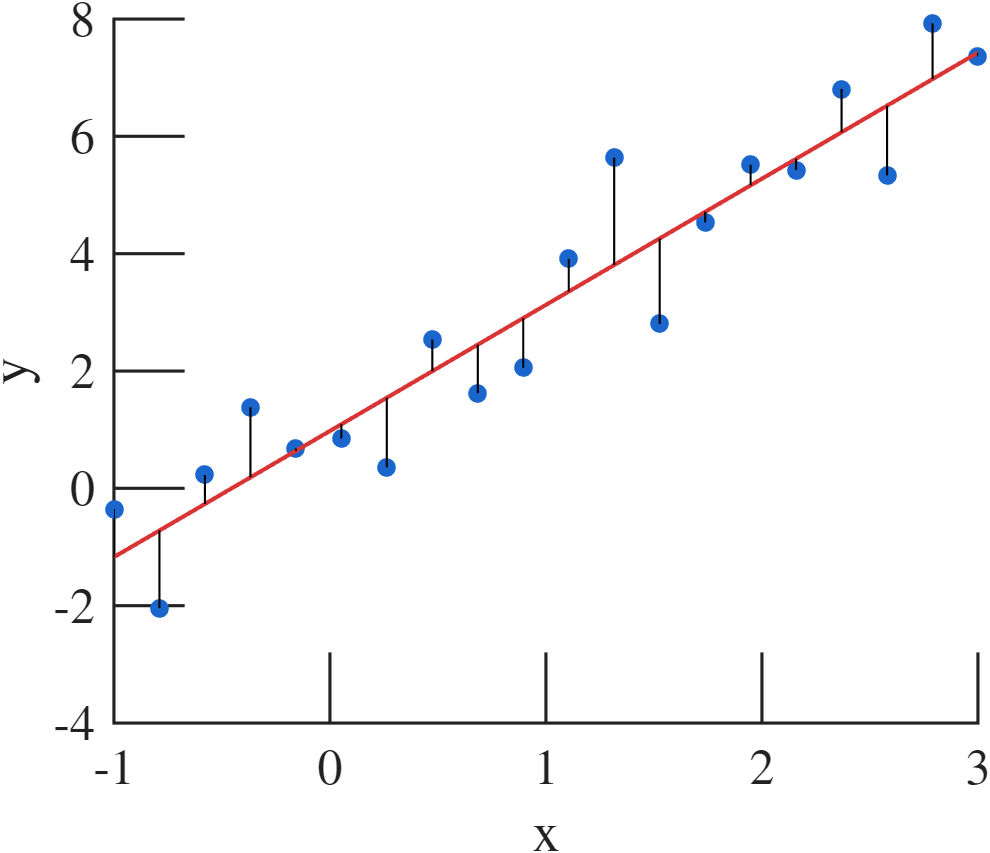
\includegraphics[width=\linewidth]{figs/scatter4.png}
    Sum of squared residuals $\|r\|_2^2=16.0863$
\end{figure}
}

\keyidea{Minimizing $\|r\|^2$ generates the line that best represents the data.}
\end{frame}
%%%%%%%%%%%%%%%%%%%%%%%%%%%%%%%%%%%%%%%%%%%%%%%%%%%%%%%%%%%%%%%%
\sectionframe{Normal Equations}
%%%%%%%%%%%%%%%%%%%%%%%%%%%%%%%%%%%%%%%%%%%%%%%%%%%%%%%%%%%%%%%%

\begin{frame}{How do you find the optimal line?}

\begin{block}{Objective}
    Find the line of best fit $y=\alpha x+\beta$ that represents the data $(x_i,y_i)$.
\end{block}
\vfill 
\begin{block}{Least Squares}
    Find the \textbf{least} value of the sum of \textbf{squares} $E = \sum_i(y_i - (\alpha x_i+\beta))^2$
\end{block}
\vfill 

\onslide<2>{
\question{How do we accomplish this algorithmically?}

}
\vfill 

\end{frame}

%%%%%%%%%%%%%%%%%%%%%%%%%%%%%%%%%%%%%%%%%%%%%%%%%%%%%%%%%%%%%%%%

\begin{frame}{Optimization}

\begin{itemize}
    \item Suppose you want to find the local minimum of $y=f(x)$
        \vfill

    \item First, find $f'(x)$
        \vfill

    \item Set $f'(x)=0$ and then solve for $x$
        \vfill

    \item A stationary point is a candidate; check that it is a minimum
        \vfill
    \item<2> For least squares, the objective is convex: every stationary point is a global minimum.
\end{itemize}
    
\end{frame}

%%%%%%%%%%%%%%%%%%%%%%%%%%%%%%%%%%%%%%%%%%%%%%%%%%%%%%%%%%%%%%%%

\begin{frame}{Least Squares}
\begin{itemize}
 
    \item We can express $\| r\|_2^2$ in terms of $x$:
    $$||r||^2_2 = r^Tr = (b-Ax)^T(b-Ax) = \underbrace{b^Tb - 2x^TA^Tb + x^TA^TAx}_{\phi(x)}$$

\item Take the gradient and set it to zero: $\nabla\phi(x)=0$.  
 $$\nabla\phi(x) = -2A^Tb+  2A^TAx = 0$$

\item Rearrange 
\begin{align*}
       2A^TAx &= 2A^Tb\\
       A^TAx &= A^Tb
\end{align*}

\define{Normal Equations}{
For a system $Ax=b$, the {\bf{normal equations}} are defined to be $$A^TAx = A^Tb.$$ 
}

\end{itemize}
\end{frame}


%%%%%%%%%%%%%%%%%%%%%%%%%%%%%%%%%%%%%%%%%%%%%%%%%%%%%%%%%%%%%%%%%%%%%

%%%%%%%%%%%%%%%%%%%%%%%%%%%%%%%%%%%%%%%%%%%%%%%%%%%%%%%%%%%%%%%%%%%%%
\begin{frame}{Summary of Least Squares}

\begin{enumerate}

    \item An overdetermined system need not have an exact solution 
        $$Ax=b$$
    
    \item We can find the line of best fit \bigskip 

        Minimize the sum of squared residuals $\|r\|_2^2$ \bigskip

    \item This amounts to solving the normal equations 
        $$A^TAx = A^Tb $$ 
\end{enumerate}
Advantages: 
\begin{itemize}
    \item Well-defined problem 
    \item $A^TA$ is invertible if and only if $A$ has full column rank
    \item With full column rank, $A^TA$ is symmetric positive definite, so CG applies
\end{itemize}
    
\end{frame}

%%%%%%%%%%%%%%%%%%%%%%%%%%%%%%%%%%%%%%%%%%%%%%%%%%%%%%%%%%%%%%%%%%%%%%%%
\begin{frame}{Example}
\begin{example}
    Find the line of best fit for the data points $(-3,-2)$, $(1,0)$, $(2,4)$. 
\end{example}
\begin{itemize}
    \item Let the fit be $y=\alpha x + \beta$ 

    \item Then the system is 
    $$
    \begin{aligned}
        -2 &= -3\alpha + \beta\\
        0 &= \alpha + \beta \\
        4 &= 2\alpha + \beta
    \end{aligned} \quad \implies \begin{bmatrix}
            -3 & 1\\
            1 & 1\\
            2 & 1
        \end{bmatrix} \begin{bmatrix}
            \alpha\\\beta
        \end{bmatrix}= \begin{bmatrix}
            -2\\0\\4
        \end{bmatrix}
    $$
    \item Calculate $A^TA =\begin{bmatrix}
            -3 & 1 & 2\\
            1 & 1 & 1
        \end{bmatrix} \begin{bmatrix}
            -3 & 1\\
            1 & 1\\
            2 & 1
        \end{bmatrix}  =\begin{bmatrix}
        14 & 0\\0 & 3
    \end{bmatrix}$ 
    
    \item Calculate $A^Tb=\begin{bmatrix}
            -3 & 1 & 2\\
            1 & 1 & 1
        \end{bmatrix}\begin{bmatrix}
            -2\\0\\4
        \end{bmatrix}=\begin{bmatrix}
        14\\2
    \end{bmatrix}$

\end{itemize}
\end{frame}

%%%%%%%%%%%%%%%%%%%%%%%%%%%%%%%%%%%
\begin{frame}{Example}

\begin{itemize}

    \item The normal equations are $A^TAx=A^Tb$: 
    $$
    \begin{bmatrix}
        14& 0\\
        0 & 3
    \end{bmatrix} \begin{bmatrix}
        \alpha\\\beta
    \end{bmatrix} = \begin{bmatrix}
        14\\2
    \end{bmatrix}
    $$
    \item Solving the system gives
    $$\alpha = 1,\quad \beta = 2/3$$

    \item The line of best fit is 
    $$
        y = x+\frac23
    $$
\end{itemize}
\end{frame}
\begin{frame}{Example}

\begin{figure}
    \centering
    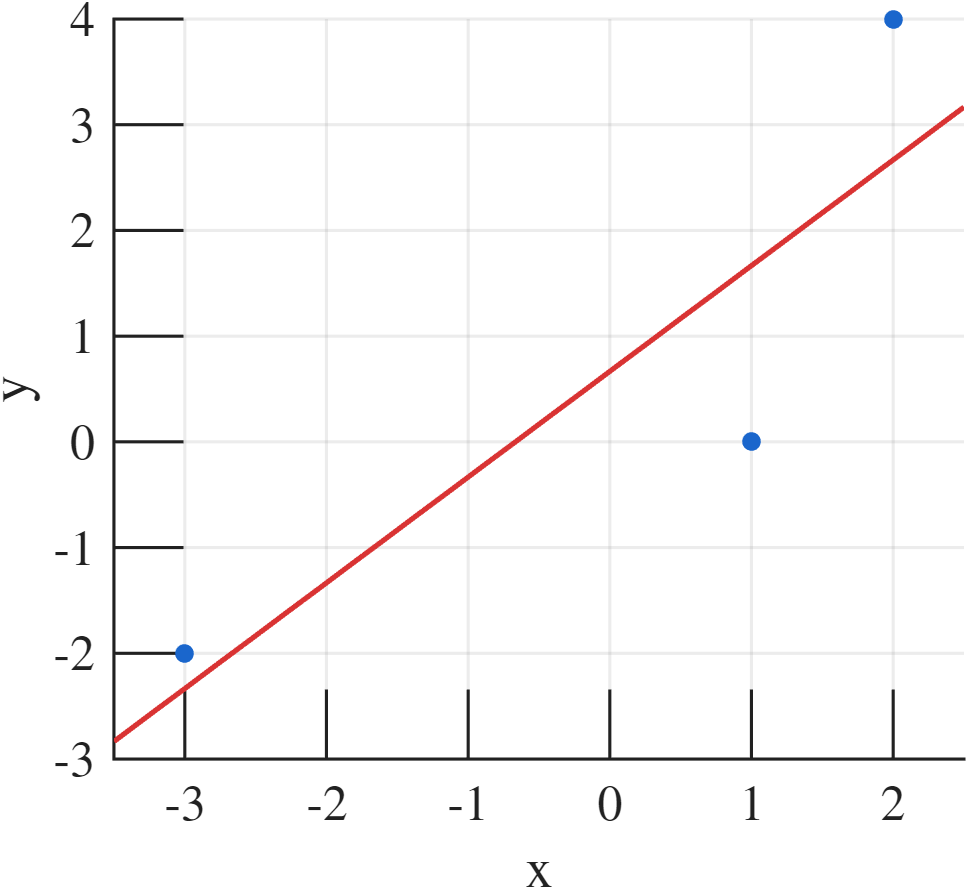
\includegraphics[width=0.5\linewidth]{figs/regexample.png}
\end{figure}
    \begin{example}
    Line of best fit for $(-3,-2)$, $(1,0)$, $(2,4)$ is $y=x+\frac23$. 
\end{example}
\end{frame}


%%%%%%%%%%%%%%%%%%%%%%%%%%%%%%%%%%%%%%%%%%%%%%%%%%%%%%%%%%%%%%%%%%
% \begin{frame}
% \frametitle{Solving normal equations}

% \begin{itemize}
%     \item 
% Since the normal equations forms a symmetric positive definite system, we can solve by computing the Cholesky factorization $$A^TA = LL^T$$ and solving $Ly = A^Tb$ and $L^Tx = y$.     

% \bigskip

% Consider 
% \[A = 
% \begin{bmatrix}
% 1 & 1 \\ 
% \epsilon & 0 \\
% 0 & \epsilon
% \end{bmatrix}
% \]
% where $0 < \epsilon < \sqrt{\epsilon_{mach}}$.  
% The normal equations for this system is given by 
% \[A^TA = \begin{bmatrix}
% 1+\epsilon^2 & 1 \\
% 1 & 1+\epsilon^2
% \end{bmatrix} = 
% \begin{bmatrix}
% 1 & 1 \\
% 1 & 1
% \end{bmatrix}
% \]
% \end{itemize}
% \end{frame}
%%%%%%%%%%%%%%%%%%%%%%%%%%%%%%%%%%%%%%%%%%%%%%%%%%%%%%%%%%%%%%%%%%%%%%%%
%%%%%%%%%%%%%%%%%%%%%%%%%%%%%%%%%%%%%%%%%%%%%%%%%%%%%%%%%%%%%%%%%%%%%%%%
\begin{frame}[fragile]{An issue...}
Disadvantage:

\begin{itemize}
    \item  The normal equations tend to worsen the condition of the matrix. 

\begin{theorem}
For full-column-rank $A$, in the 2-norm:
$$\kappa_2(A^TA)=\kappa_2(A)^2.$$
\end{theorem}
\item Recall that $cond(A)\ge1$ 

\begin{lstlisting}
>> A = rand(10,10);
>> cond(A)
   43.4237
>> cond(A'*A)
   1.8856e+03
\end{lstlisting}

\end{itemize}

\keyidea{
Forming the normal equations squares the condition number. QR or SVD avoids this extra loss of numerical accuracy.
}

\end{frame}
%%%%%%%%%%%%%%%%%%%%%%%%%%%%%%%%%%%%%%%%%%%%%%%%%%%%%%%%%%%%%%%%%%%%
% \begin{frame}{Normal Equations are not good enough}
% \begin{center}
%     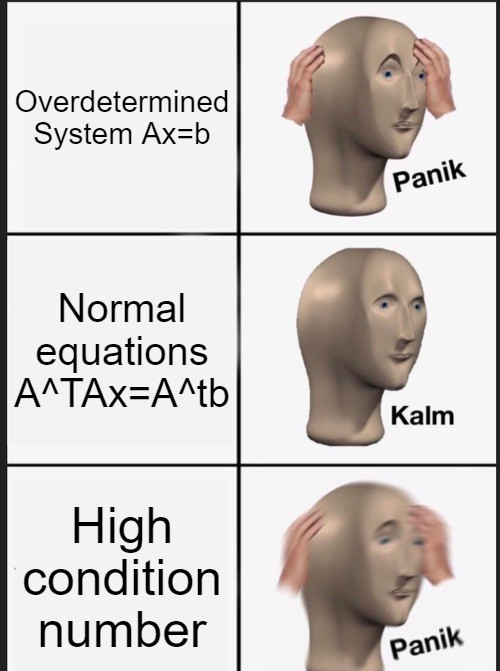
\includegraphics[scale=0.4]{figs/meme-normal_eq.jpg}
% \end{center}
    
% \end{frame}
%%%%%%%%%%%%%%%%%%%%%%%%%%%%%%%%%%%%%%%%%%%%%%%%%%%%%%%%%%%%%%%%%%%%

\sectionframe{Least Squares with SVD}

%%%%%%%%%%%%%%%%%%%%%%%%%%%%%%%%%%%%%%%%%%%%%%%%%%%%%%%%%%%%%%%%%%%%

% \begin{frame}{Other approaches}
% How can we solve the least squares problem without squaring the condition of the matrix?
% \\\bigskip
% Utilize factorizations that involve orthogonal matrices: \bigskip
% \begin{itemize}
% \item $QR$ factorization: $A = QR$ where 
% \begin{itemize}
% \item $Q$ is an $m\times m$ orthogonal matrix 
% \item $R$  is an $m\times n$ upper triangular matrix (since $R$ is an $m\times n$ upper triangular matrix we can write $R = \begin{bmatrix} R' \\ 0 \end{bmatrix}$ where $R$ is $n\times n$ upper triangular and 0 is the $(m-n) \times n$ matrix of zeros)
% \end{itemize}

% \bigskip

% \item SVD:  $A = U\Sigma V^T$ where 
% \begin{itemize}
% \item $U$ is an $m\times m$ orthogonal matrix
% \item $V$ is an $n\times n$ orthogonal matrix
% \item $S$ is an $m\times n$ diagonal matrix whose elements are the singular values.
% \end{itemize}
% \end{itemize}

% \end{frame}

%%%%%%%%%%%%%%%%%%%%%%%%%%%%%%%%%%%%%%%%%%%%%%%%%%%%%%%%%%%%%%%%%%%%%%%%
%%%%%%%%%%%%%%%%%%%%%%%%%%%%%%%%%%%%%%%%%%%%%%%%%%%%%%%%%%%%%%%%%%%%%%%%
    % \begin{frame}{Using QR Factorization in Least Squares}
    % \begin{itemize}
    %     \item We still want to minimize $ \|r\|^2_2$
    %     \item Let's rewrite the least square equation using QR
    %     \begin{align*}
    %     \|r\|^2_2 &= \|b-Ax\|^2_2 = \left\|b-Q \begin{bmatrix} R \\ 0 \end{bmatrix}x\right\|^2_2 \\ 
    %     &= \left\|Q^Tb - Q^TQ\begin{bmatrix}R \\ 0 \end{bmatrix}x \right\|^2_2 = \left\|Q^Tb - \begin{bmatrix} R \\ 0 \end{bmatrix}x \right\|^2_2
    %     \end{align*}
    % \item Let $Q^Tb = \begin{bmatrix} v_1  \\ \hline v_2 \end{bmatrix}$.  Then 
    % $$\left\|Q^Tb-\begin{bmatrix}R\\0\end{bmatrix} x \right\|^2_2 = \left\|\begin{bmatrix}v_1\\v_2\end{bmatrix} - \begin{bmatrix} Rx \\0\end{bmatrix}\right\|^2_2 = \left\|\begin{bmatrix} v_1-Rx \\ v_2 \end{bmatrix}\right\|^2_2 = ||v_1 - Rx||^2_2 + ||v_2||^2_2$$ 
    
    % \item We simply solve $R x  = v_1 $ (upper triangular system) 
    
    % \end{itemize}
    % \end{frame}
    
    % \begin{frame}{The QR Least Squares Method}
    % \method{QR Least Squares}{Overdetermined system $Ax=b$}{Best approximate solution $\tilde{x}$}{The factorization $A=QR$ let's us avoid the ill-conditioned normal equations.}
    
    % \begin{itemize}
    %     \item $cond(A^TA)$ has a high condition number
    %     \item QR factorization lets us avoid the normal equations
    %     \item Can find $A=QR$ with \textbf{Gram-Schmidt orthogonalization}.
    % \end{itemize}
    
    % If $A=QR$ then $span(A) = span(Q)$. We can construct $Q$ by doing Gram-Schmidt on the columns of $A$.
    % \end{frame}
%%%%%%%%%%%%%%%%%%%%%%%%%%%%%%%%%%%%%%%%%%%%%%%%%%%%%%%%%%%%%%%%%%%%%%%%

%%%%%%%%%%%%%%%%%%%%%%%%%%%%%%%%%%%%%%%%%%%%%%%%%%%%%%%%%%%%%%%%%%%%%%%%
    % \begin{frame}
    % \frametitle{Gram-Schmidt orthogonalization}
    % \begin{itemize}
    %     \item $R$ is upper triangular and $A = QR$. We can write out the columns of $A$: 
    % \begin{eqnarray*}
    % a_1 &=& q_1r_{11} \\
    % a_2 &=& q_1r_{12} + q_2r_{22} \\
    % \vdots &=& \quad \vdots \\
    % a_n &=& q_1r_{1n} + q_2r_{2n} + ... + q_nr_{nn}
    % \end{eqnarray*}
    % \item We can leverage the orthogonality of the $q$ vectors to write 
    % $$r_{ij} = q_i^T a_j, j>i$$
    % \begin{block}{Key Idea}
    % There is a lot of overlap between the construction of $R$ and the Gram-Schimdt. It is not efficient to do them separately. $\implies$ Do both at the same time. 
    % \end{block}
    % \end{itemize}
    % \end{frame}
    
%%%%%%%%%%%%%%%%%%%%%%%%%%%%%%%%%%%%%%%%%%%%%%%%%%%%%%%%%%%%%%%%%%%%%%%%
 
    % \begin{frame}[fragile]
    % \frametitle{Gram-Schmidt QR Factorization}
    
    % \begin{lstlisting}
    % function [Q,R] = gs_qr (A)
    
    % m = size(A,1);
    % n = size(A,2);
    
    % for i = 1:n 
    %     R(i,i) = norm(A(:,i),2);
    %     Q(:,i) = A(:,i)./R(i,i);
    %     for j = i+1:n
    %         R(i,j) = Q(:,i)' * A(:,j);
    %         A(:,j) = A(:,j) - R(i,j)*Q(:,i);
    %     end
    % end
    
    % end
    % \end{lstlisting}
    % \bigskip
    % This algorithm constructs $R$ and does the Gram-Schmidt at the same time.
    % \end{frame}
    
%%%%%%%%%%%%%%%%%%%%%%%%%%%%%%%%%%%%%%%%%%%%%%%%%%%%%%%%%%%%%%%%%%%%%%%%
%%%%%%%%%%%%%%%%%%%%%%%%%%%%%%%%%%%%%%%%%%%%%%%%%%%%%%%%%%%%%%%%%%%%%%%%
% \begin{frame}{Recap}

% \begin{itemize}
%     \item The goal is to find the line of best fit $y=c_1x+ c_0 $ 
%     \bigskip 
%     \item \textbf{Least squares problem}: solve $Ax=b$, ($A$ is $n\times 2$) such that the square of the residual $||r||^2_2$ = $||b-Ax||^2_2$ is made least
%     \bigskip
%     \item \textbf{Normal equations}: problem can be alternatively expressed as solving $A^TAx=b$, but $A^TA$ has a high condition number
%     \bigskip 
%     \item \textbf{QR Least Squares}: Factor $A=QR$. Finding the least squares becomes a triangular system. 
%     \bigskip 
% \end{itemize}
%   We can also factor $A = U\Sigma V^T$... turns out that this is even better.
% \end{frame}
%%%%%%%%%%%%%%%%%%%%%%%%%%%%%%%%%%%%%%%%%%%%%%%%%%%%%%%%%%%%%%%%%%%%%%%%
% Full-column-rank case is the main lecture path.
\begin{frame}{Using SVD for Least Squares}
Let $A\in\mathbb{R}^{m\times n}$ have full column rank, with $m\ge n$.
\[
A=U\Sigma V^T,
\qquad U\in\mathbb{R}^{m\times m},\quad
\Sigma\in\mathbb{R}^{m\times n},\quad V\in\mathbb{R}^{n\times n}.
\]
\begin{itemize}
\item Orthogonal matrices preserve the Euclidean norm.
\item Change coordinates: $c=U^Tb$ and $y=V^Tx$.
\end{itemize}
\[
\|b-Ax\|_2^2
=\|U^Tb-\Sigma V^Tx\|_2^2
=\|c-\Sigma y\|_2^2.
\]
\keyidea{Rotate or reflect the coordinates: the fitting error is unchanged, but the matrix becomes diagonal.}
% Talking point: U and V change coordinates; Sigma does the scaling.
\end{frame}

\begin{frame}{Fit What We Can; Keep the Remaining Residual}
Since $\sigma_1,\ldots,\sigma_n>0$,
\[
\|c-\Sigma y\|_2^2
=\underbrace{\sum_{i=1}^n(c_i-\sigma_i y_i)^2}_{\text{we can make this zero}}
+\underbrace{\sum_{i=n+1}^m c_i^2}_{\text{unavoidable residual}}.
\]
\begin{enumerate}
\item Compute $c=U^Tb$.
\item Divide: $y_i=c_i/\sigma_i$, for $i=1,\ldots,n$.
\item Transform back: $x=Vy$.
\end{enumerate}
\keyidea{SVD avoids forming $A^TA$. Small singular values can still make the original problem sensitive.}
% Talking point: zero rows of Sigma cannot reproduce the final components of c.
\end{frame}

\begin{frame}{The SVD Least-Squares Solution}
For full-column-rank $A$, the unique least-squares solution is
\[
\boxed{x=\sum_{i=1}^n\frac{u_i^Tb}{\sigma_i}v_i.}
\]
\begin{itemize}
\item Project the data onto each $u_i$.
\item Divide by the corresponding singular value.
\item Combine the right singular vectors $v_i$.
\end{itemize}
% Main lecture path: continue to polynomial fitting if short on time.
\end{frame}

\begin{frame}{Reference: Rank-Deficient Least Squares}
If $\operatorname{rank}(A)=r<n$, only $\sigma_1,\ldots,\sigma_r$ are positive:
\[
\|c-\Sigma y\|_2^2
=\sum_{i=1}^r(c_i-\sigma_i y_i)^2+\sum_{i=r+1}^m c_i^2.
\]
\begin{itemize}
\item Set $y_i=c_i/\sigma_i$ for $i\le r$.
\item The other coordinates do not affect the residual.
\item Choose $y_{r+1}=\cdots=y_n=0$ for the smallest solution norm.
\end{itemize}
\[
\boxed{x_{\min}=\sum_{i=1}^r\frac{u_i^Tb}{\sigma_i}v_i.}
\]
% Optional reference slide: least-squares solutions need not be unique,
% but the solution with minimum Euclidean norm is unique.
\end{frame}
%%%%%%%%%%%%%%%%%%%%%%%%%%%%%%%%%%%%%%%%%%%%%%%%%%%%%%%%%%%%%%%%%%%%%%%%
\sectionframe{Other Fitting}
%%%%%%%%%%%%%%%%%%%%%%%%%%%%%%%%%%%%%%%%%%%%%%%%%%%%%%%%%%%%%%%%%%%%%%%%
\begin{frame}{Fitting a Quadratic}
    \begin{center}
    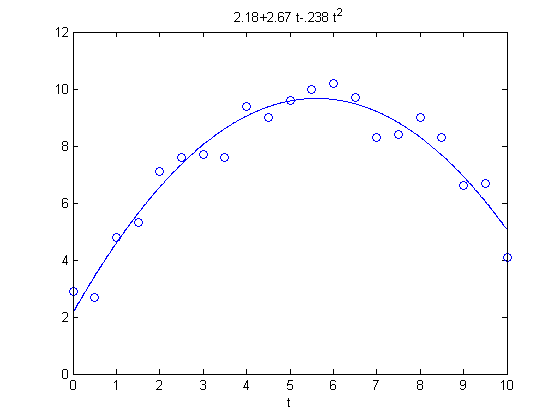
\includegraphics[width=8cm]{figs/lsquadratic.png}\\
    How can we find the quadratic of best fit?
    \end{center}
\end{frame}
%%%%%%%%%%%%%%%%%%%%%%%%%%%%%%%%%%%%%%%%%%%%%%%%%%%%%%%%%%%%%%%%%%%%%%%%
\begin{frame}{Fitting a Quadratic}
\begin{itemize}
\item Let's assume our data is quadratic $y = a + b x + cx^2 $\bigskip
    
\item Our given data points are 
\begin{align*}
(x_1&,y_1)\\
(x_2&,y_2)\\
&\vdots\\
(x_n&,y_n)
\end{align*}

\item Our interpolation system would be 
\begin{align*}
y_1&= a+bx_1+cx_1^2\\
y_2&= a+bx_2+cx_2^2\\
&\vdots\\
y_n&= a+bx_n+cx_n^2
\end{align*}


\end{itemize}
\end{frame}
%%%%%%%%%%%%%%%%%%%%%%%%%%%%%%%%%%%%%%%%%%%%%%%%%%%%%%%%%%%%%%%%%%%%%%%%
\begin{frame}{Fitting a Quadratic}
\begin{itemize}
\item For $n>3$, this is a rectangular \textit{Vandermonde matrix}
$$ \underbrace{\begin{bmatrix}  1& x_1&x_1^2 \\ \vdots & \vdots & \vdots \\
1 & x_n & x_n^2 \end{bmatrix}}_A 
\underbrace{\begin{bmatrix}a \\ b \\ c \end{bmatrix}}_{x} 
= 
\underbrace{\begin{bmatrix} y_1 \\ \vdots \\ y_n \end{bmatrix}}_{b}$$
\item For more than three data points this is overdetermined. Least-squares solutions satisfy the normal equations
$$
A^TAx = A^Tb
$$

\keyidea{

\begin{itemize}
    \item The model must be linear in its unknown coefficients
    \item Then linear least squares applies; solve with QR or SVD
\end{itemize}
}

\end{itemize}
\end{frame}
%%%%%%%%%%%%%%%%%%%%%%%%%%%%%%%%%%%%%%%%%%%%%%%%%%%%%%%

\begin{frame}{Common Regression Models}

\textbf{1. Linear Regression}
\[
  y = ax + b
\]

\medskip
\textbf{2. Quadratic Regression}
\[
  y = ax^2 + bx + c
\]

\medskip
\textbf{3. Cubic Regression}
\[
  y = ax^3 + bx^2 + cx + d
\]

\medskip
% \textbf{4. Exponential Regression}
% \[
%   y = Ce^{kx}
% \]
% Often linearized by taking logarithms:
% \[
%   \ln(y) = \ln C + kx.
% \]

% \medskip
% \textbf{5. Power Law Regression}
% \[
%   y = Cx^{\,k}
% \]
% Linearize via
% \[
%   \ln(y) = \ln C + k\ln(x).
% \]

\end{frame}

% Optional extension if time permits.
\begin{frame}{Nonlinear Models}

\question{What do you do if your data appears to be exponential?}
    \begin{figure}
        \centering
        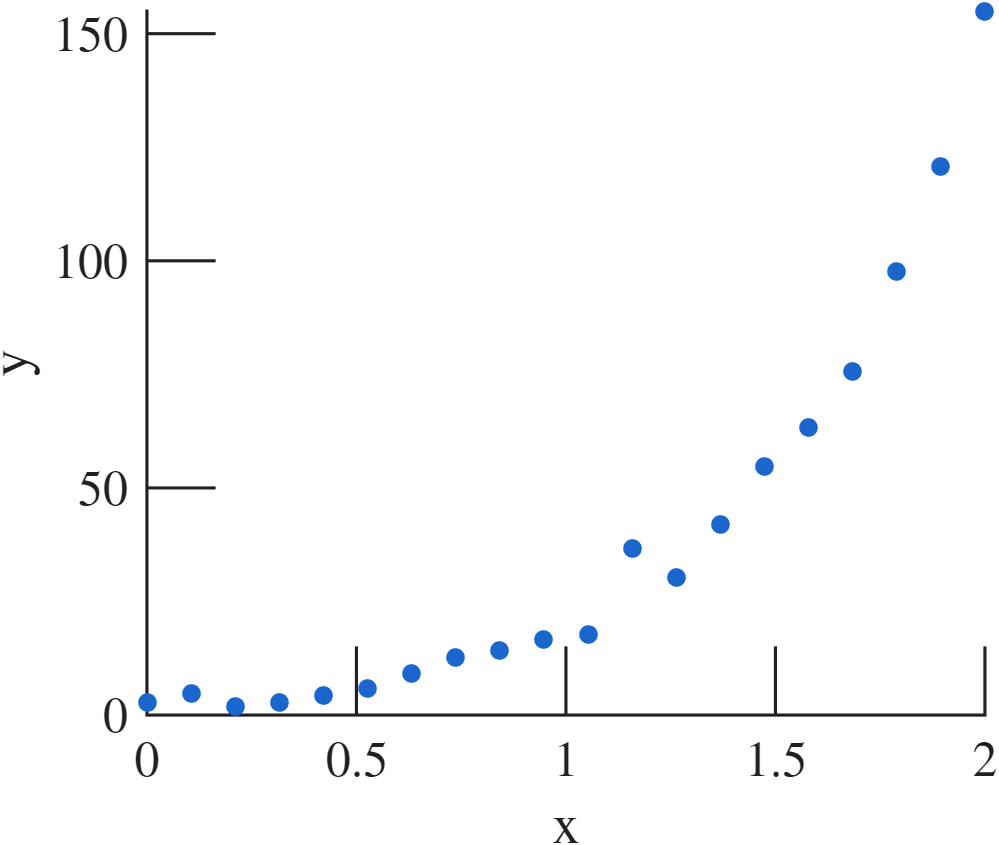
\includegraphics[width=0.5\linewidth]{figs/scatter5.png}
    \end{figure}

    \begin{itemize}
        \item There's an issue with the model 
        $$y = ae^{bx}$$
    \end{itemize}
\end{frame}

\begin{frame}{Nonlinear Models}


    \begin{itemize}
        \item Fitting data on the model $y = ae^{bx}$ yields 
        \begin{align*}
y_1&= ae^{bx_1}\\
y_2&= ae^{bx_2}\\
&\vdots\\
y_n&= a e^{bx_n}
\end{align*}

    \item \textbf{Problem}: this is \textit{not} a linear system
        \vfill 
    \item For positive data and $a>0$, a log transformation is possible
        $$
        \ln(y) = \ln(ae^{bx}) = \ln a + bx
        $$
    \end{itemize}
\end{frame}

%%%%%%%%%%%%%%%%%%%%%%%%%%%%%%%%%%%%%%
\begin{frame}{Transform the Data}

\begin{figure}
    \centering
    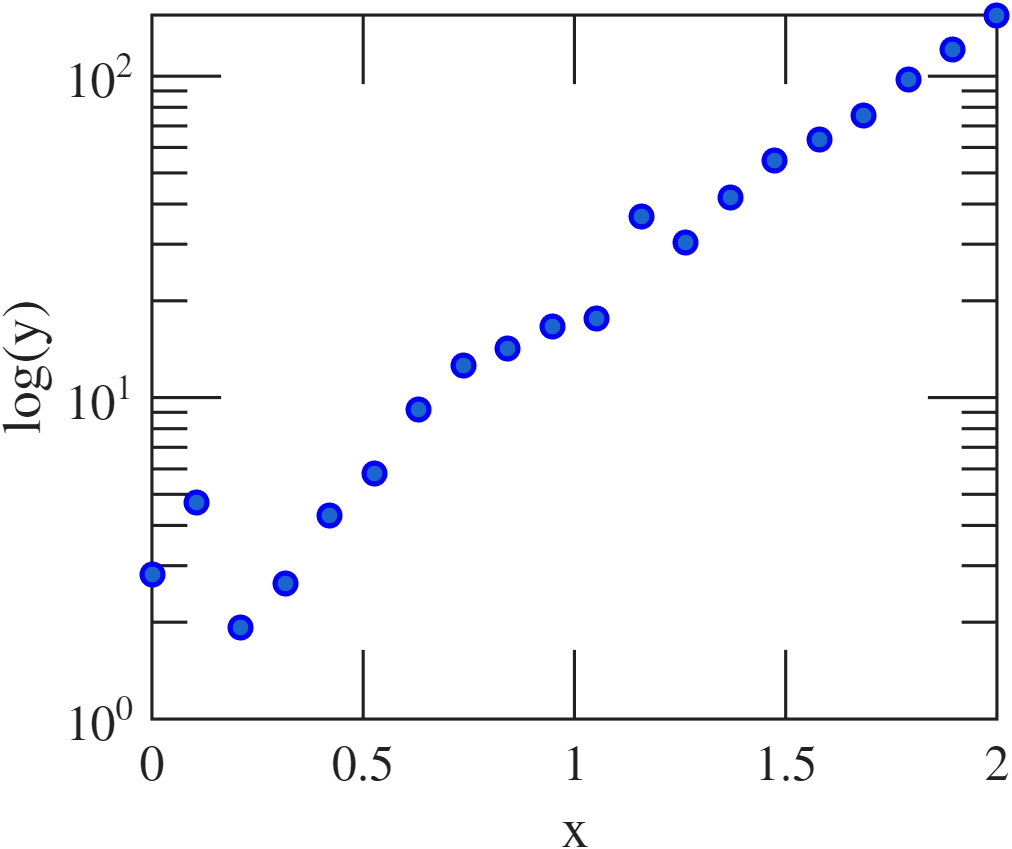
\includegraphics[width=0.45\linewidth]{figs/scatter6.png}
    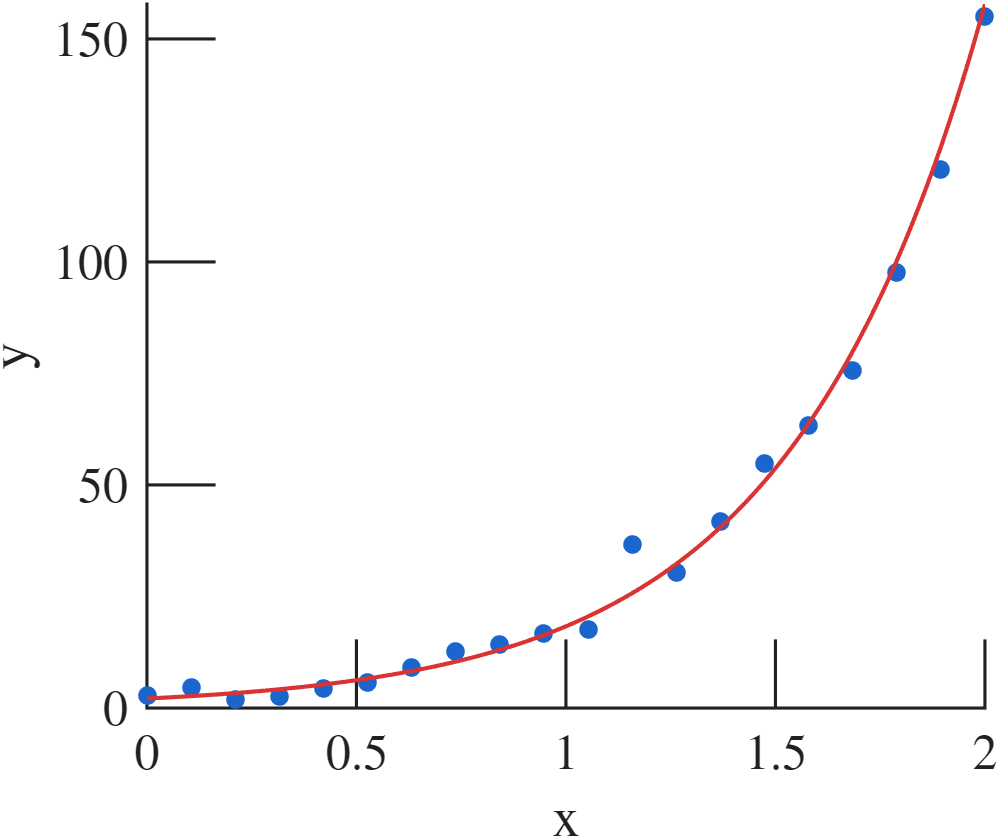
\includegraphics[width=0.45\linewidth]{figs/scatter7.png}
\end{figure}

\begin{itemize}
    \item Fit the data on $$\ln(y) = \ln a + bx$$
    \item This minimizes squared errors in $\ln y$, not in $y$.
    \item Undo the transformation
    $$
    y = ae^{bx}
    $$
\end{itemize}
    
\end{frame}


\begin{frame}{Summary}
    \begin{itemize}
        \item Fitting a model linear in its coefficients often gives an overdetermined system
        $$
        Ax=b,
        $$
        where $A$ is $m\times n$ and $m$ is much larger than $n$
            \vfill 
        \item We can instead solve 
        $$
        A^TAx = A^Tb
        $$
        to find the "best-fit" equation
        \vfill 
        \item In practice, use QR or SVD; with $A=U\Sigma V^T$, minimize
                $$ \|\Sigma V^Tx-U^Tb\|_2^2. $$

    \end{itemize}
\end{frame}
% \begin{frame}{Experiment}
%     \begin{itemize}
%         \item Choose a random quadratic $y = f(x) = 3x^2 -7x +2 $
%         \item Choose an interval, say $[-1,1]$, and sample points $n$ points. 
%         \item You have a set of $n$ data points $(x_i,y_i)$ 
%         \item Now artificially add noise to the data $y_i$
%         \begin{alertblock}{Question}
%             Can you recover the coefficients 3, -7, and 2 by doing least squares?
%         \end{alertblock}
%     \end{itemize}

    
% \end{frame}

%%%%%%%%%%%%%%%%%%%%%%%%%%%%%%%%%%%%%%%%%%%%%%%%%%%%%%%%%%%%%%%%%%%%%%%%


\end{document}
